
\section{Introducing Java}
\label{sec:introducing-java}

The time has come to start using full-flavoured Java. This section
will introduce the main features that are new with respect to what we
have seen so far. We will make a gradual transition to the new
language. 

\subsection{Everything is a class}
\label{sec:everything-class}

In Java all the code comes inside a class. There is no class-less
code as in Groovy. 

Usually every class is defined in its own file, e.g.~a \verb+Person+
class is defined in a file called \verb+Person.java+. When a file
contains only one class, this class must be public and have the same
name as the file (without the \verb+.java+ extension). 

Classes in different files must be compiled independently before they
can be used. This is another important difference with the Groovy
scripts we have been using until now, where every script was
self-contained. From now on we will have classes in different files,
and unless we compile\footnote{If you do not remember clearly what
  \emph{compiling} means, read again the notes from day 1. } them and
transform those text files into something that can be understood by
the machine, the machine will not find the classes you are
calling. Java classes (i.e.~files) are compiled with the java
compiler, \verb+javac+. 

\begin{verbatim}
    > javac Person.java
\end{verbatim}

This will produce a file \verb+Person.class+ in your folder. Once you
have it, you can use the Person class from any other file. 

\paragraph{Classpath. }
\label{sec:classpath.-}

You may be wondering how is it possible to use classes like String
that are not in your current directory in the form of a \verb+.class+
file. This is because Java comes with a lot of classes built-in,
including String. These classes are in your CLASSPATH, which is a list
of locations in your computer\footnote{A CLASSPATH is something
  conceptually similar to a PATH, a list of locations in your computer
  where the operating system looks for executable files when you type
  them in the command line. Both are environment variables, and can be
  accessed and modified in the same way.} where Java looks for the
classes you are using in your program. We will see more about this in
the future.

\subsection{The Java Library}
\label{sec:java-api}

Java is not just a programming language (a set of keywords and
syntactic rules). It provides as well a broad library of classes that
you can use in your program. Some of them you know them already, like
String, or the boxed types (Integer, Double, etc). 

This library is available for any Java programmer for free. There are
literally thousands of useful classes in the library, and they are
well documented in one website, coloquially referred to as ``the
JavaDoc''. You can find it very easily by using your favourite search
engine to look up ``java API'' (Figure~\ref{fig:ajavadoc}). API stands
for Application Programmer's Interface. 

\begin{figure}[tbhp]
  \centering
  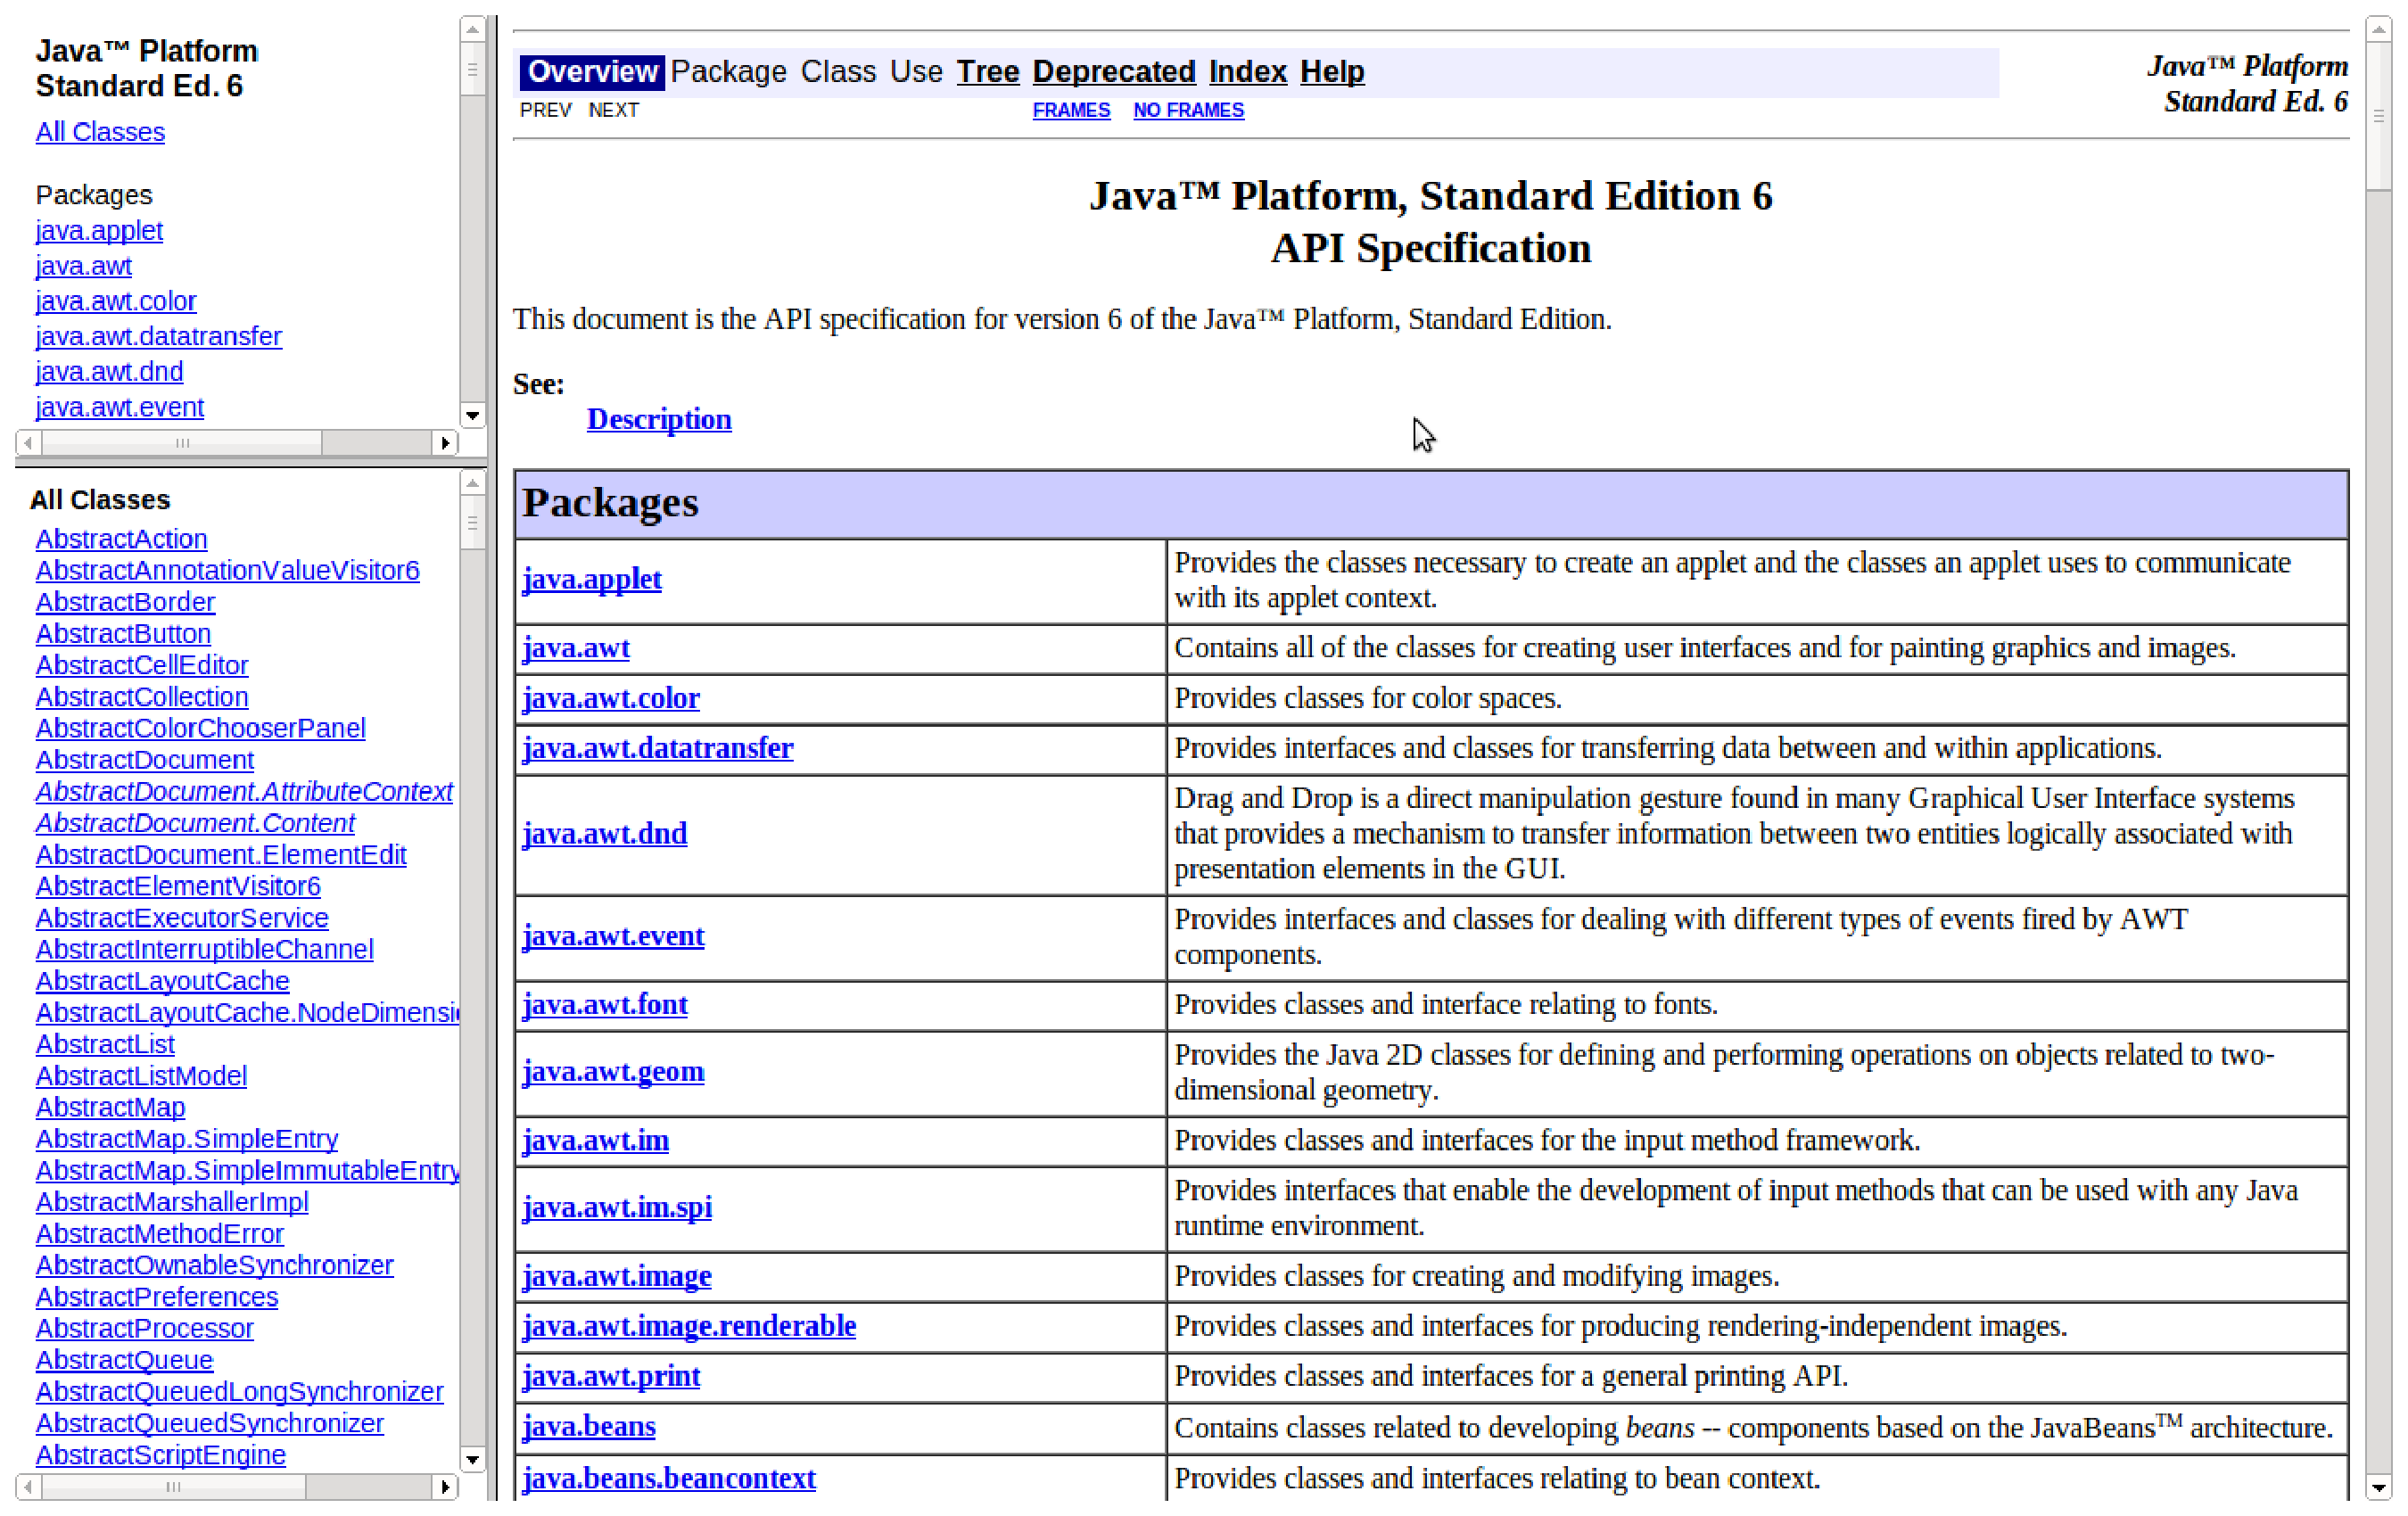
\includegraphics[width=\textwidth]{gfx/javadoc}
  \caption{The Java API main page}
  \label{fig:ajavadoc}
\end{figure}

You can see that there are three frames: top-left, a list of packages
(we will learn what packages are at a later point); bottom-left, a
list of classes; right, the main frame. You can find a lot of
information about all classes in the Java Library on this website. You
can also get a local copy if you plan to work without an internet
connection. 

Look up any class (e.g.~String) in the list of classes at the
bottom-left. Click on it. Read the documentation on the main
frame. Every page in Java Doc follows the same structure: 

\begin{description}
\item[General description: ] at the beginning.
\item[List of fields: ] all visible fields of the class, if any.
\item[List of constructor methods: ] each of them with a brief
  description, a list of parameters and other useful information, and
  a link to a more detailed description.
\item[List of methods: ] each of them with a brief
  description, a list of parameters and other useful information, and
  a link to a more detailed description.
\item[Detailed description of methods. ] 
\end{description}

You must become familiar with the Java Doc. You will use it very often
as a Java programmer. 

% \subsection{A new type of loop: do\ldots while}
% \label{sec:new-type-loop}



%%% Local Variables:
%%% mode: latex
%%% TeX-master: "main"
%%% End:
